\section{Tensor Operations and \einsum}
\label{sec:preliminary}

In this section, we outline multi-linear operations common to TNNs. Many of these operations are systematically expressible and computable via the popular notational framework and function \einsum, first introduced by the Python library \numpy~\citep{harris2020array}.
Therefore, we will first review the most important tensor network operations and their corresponding \einsum representations. With these concepts in hand, we then formally introduce TNN.

\textbf{Notations.}
We use lower case letters (e.g., $\myvector{v}$) to denote vectors, 
upper case letters (e.g., $\mymatrix{M}$) denote matrices, 
and curly letters (e.g., $\mytensor{T}$) denote tensors.
For a tensor $\mytensor{T} \in \R^{I_1 \times I_2 \times \cdots \times I_N}$, we refer to a specific entry by the subscript notation $T_{i_1 i_2 \dots i_N}$, where $1 \leq i_n \leq I_n$ for $1 \leq n \leq N$.
Furthermore, we refer to $N$ as the order, a particular index $n$ as a mode, and the magnitude of a mode $I_n$ as dimension size.
For example, a tensor $\mytensor{T} \in \R^{3 \times 4 \times 5}$ is a $3^\rd$ order tensor that has dimension size $4$ at its second mode.

\subsection{Representations of Multilinear Operations}
\label{sub:multi-ops}

The \einsum function allows definitions of multilinear operations via string inputs. In this subsection, we highlight an example of a multilinear operation involving three primitive operations ({\em contraction}, {\em batch product}, {\em outer product}) in the language of \einsum.
% simultaneous operations between two tensors
Consider two $3^\rd$-order tensors $\tensorSup{T}{1} \in \R^{B \times C \times I}$, $\tensorSup{T}{2} \in \R^{A \times R \times T}$, and a multilinear operation between these two tensors:
\begingroup
\abovedisplayskip=5pt
\belowdisplayskip=5pt
\begin{equation}
\label{eq:multi-operation}
\tensorSub{T}{b,i,j} = \sum_{c = 1}^{C}
\tensorInd{T}{1}{b,c,s} \tensorInd{T}{2}{b,c,j}.
\end{equation}
\endgroup
We can denote the operation above in \einsum as:
\begin{lstlisting}
T = einsum("bci,bcj->bij", T1, T2)
\end{lstlisting}
\vspace{-1em}
where the string in the quotation mark precisely specifies the operation, which is known as an \einsum string. In this string, the letter \textsf{"c"} indicates {\em contraction} since it appears in both inputs but not the output; the letter \textsf{"b"} denotes {\em batch product} since it appears in both inputs and the output; lastly, the letters \textsf{"i"} and \textsf{"j"} represent {\em outer product} as they each appears in one of the two inputs and they both appear in the output. %Note that any letter in an \einsum string falls into one of these three classes (except for the trivial case that a letter appearing in only one input or output). 
A detailed description of \einsum and definitions of these operations is provided in \Cref{app:subsec:einsum}.

\subsection{From \einsum to \conveinsum}
\label{sub:einsum}
While many popular libraries (e.g., \numpy, \textsf{TensorFlow}, \pytorch) implement \einsum, none of them support convolutions, despite that convolution is (multi)linear and ubiquitous in modern neural networks.
We therefore generalizes \einsum to a meta-function \conveinsum, 
which handles convolution as a primitive operation.

{\bf Tensor convolution} generalizes the convolution on vectors to higher-order tensors thereby extending the familiar linear convolution to a multi-linear operation.
For instance, given two tensors $\tensorSup{T}{1} \in \R^{X \times B \times C}$ and $ \tensorSup{T}{2} \in \R^{L \times D \times E}$, we can define a convolution between the modes with dimension sizes $X$ and $L$. The operation returns a $5^\th$ order tensor $\mytensor{T} \in \R^{X^\prime \times B \times C \times D \times E}$, with its entries calculated as:
\begingroup
\abovedisplayskip=5pt
\belowdisplayskip=5pt
\begin{equation}
\label{eq:convolution}
\tensorSub{T}{\slice,b,c,d,e} = 
\tensorInd{T}{1}{\slice,b,c} \ast
\tensorInd{T}{2}{\slice,d,e},
\end{equation}
\endgroup
where $\ast$ denotes a convolution between two vectors. Note that the dimension sizes $X$ and $L$ can be different, and the output dimension size $X^\prime$ depends on the convolution type (e.g., a standard convolution yields $X^\prime = X + L - 1$).
We write \Cref{eq:convolution} in our proposed \conveinsum as
\begin{lstlisting}
T = conv_einsum("lbc,lde->lbcde|l", T1, T2)
\end{lstlisting}
\vspace{-1em}
In this scheme, the same letter \textsf{"l"} is used for different modes, even if their dimension sizes may differ. Furthermore, the placement of \textsf{"l"} right to the pipe-delimiter '\textsf{|}' indicates that \conveinsum performs convolution on the corresponding modes. Notice that a letter for convolution appears in all inputs, the output, and after the delimiter.

We can use \conveinsum to represent multilinear operations on more than two inputs. For instance, consider three tensors $\mytensor{X} \in \R^{B \times F \times S \times H \times W}$, $\tensorSup{K}{1} \in \R^{F \times G \times K \times K \times K}$, $\tensorSup{K}{2} \in \R^{S \times T \times K \times K}$, and an operation
\begingroup
\abovedisplayskip=5pt
\belowdisplayskip=5pt
\begin{equation}
\tensorSub{Y}{b,g,t,\slice,\slice} = \sum_{f = 1}^{F} \sum_{s = 1}^{S} 
\tensorSub{X}{b,f,s,\slice,\slice} \ast \tensorInd{K}{1}{f,g,\slice,\slice} \ast \tensorInd{K}{2}{s,t,\slice,\slice} 
\end{equation}
which leads to an output tensor $\mytensor{Y} 
\in \R^{B \times G \times T \times H^\prime \times W^\prime}$. This is known as {\em interleaved group convolution}~\citep{zhang2017interleaved}. In \conveinsum, it writes as
\begin{lstlisting}
T = conv_einsum("bfshw,fghw,sthw->bgthw|hw",X, K1, K2)
\end{lstlisting}
\vspace{-1em}
We will discuss how to evaluate a \conveinsum with more than two inputs in \Cref{sub:algorithms-sequencer}.

\subsection{Compact Neural Networks via \conveinsum}
\label{sub:TNN}
 
In this part, we formulate various layers of compact neural networks in terms of \conveinsum.

\textbf{Standard convolution layer.} 
% We first review two of the most popular layer types, namely {\em fully-connected layers} and {\em 2D convolution layers}.
% % fully-connected layer
% {\bf (1)} A fully-connected layer is parameterized by a matrix $\mymatrix{W} \in \R^{T \times S}$, which maps a vector $\myvector{x} \in \R^{S}$ to an output vector $\myvector{y} \in \R^{T}$:
% \begin{lstlisting}
% Y = conv_einsum("bs,ts->bt", X, W)
% \end{lstlisting}
% \vspace{-1em}
% Since a neural network typically computes its inputs in mini-batches, the \einsum string contains an additional letter \textsf{"b"} to index examples in a mini-batch.
% 2D-convolutional layer
We review a popular layer type in neural networks --- the standard 2D-convolutional layer.
Such a layer is parameterized by a $4^\th$ order tensor $\mytensor{W} \in \R^{T \times S \times H \times W}$, which maps a $3^\rd$ order tensor $\mytensor{X} \in \R^{S \times H^\prime \times W^\prime}$ to a $3^\rd$ order tensor $\mytensor{Y} \in \R^{T \times H^\prime \times W^\prime}$:
\begin{lstlisting}
Y = conv_einsum("bshw,tshw->bthw|hw", X, W)
\end{lstlisting}
\vspace{-1em}
Note that a neural network typically computes its inputs in mini-batches, so the \conveinsum string contains an additional letter \texttt{"b"} to index examples in a mini-batch. Since convolutional layers include fully-connected layers as a special case when $H = W = 1$, we focus on designs of convolutional layers for the remainder of this subsection.

% figure for a convolution layer
% \begin{figure}[!htbp]
    \centering
    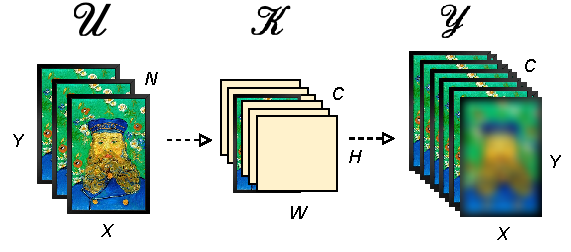
\includegraphics[width=0.45\textwidth]{\fighome/convdrawio.pdf}
    \vspace{-1.5em}
    \caption{\textbf{Depiction of a standard convolutional layer.} 
    Here $\mytensor{U} \in \R^{N\times X \times Y}$ is an $N$-stacked batch of $X\times Y$ images (Vincent van Gogh's \textit{Portrait of Joseph Roulin}). This batch is fed through a $4^\th$-order convolutional tensor $\mytensor{K}\in\R^{N \times C \times H \times W}$, where $H$ and $W$ are the kernel height and width, respectively, and $C$ is the number of output channels. (The kernel has been decomposed along its output channel mode by its matricized slices. Furthermore, we are not depicting the $N$-dimensional batch mode of each slice.) After a max-padded blurring convolution between the mode pairs $(X,H)$ and $(Y,W)$ and contraction over the $N$-dimensional batch mode, the output is a third order tensor $\mytensor{Y} \in\R^{X \times Y \times C}$.}
    \label{fig:conv-layer}
\end{figure}

\textbf{Tensorial Neural Networks.}
Convolutional layers motivate the importance and usage of TNNs since their structure has been shown to benefit from reshaping and tensorial decomposition. Numerous works propose to design {\em tensorial layers} where the (reshaped) convolution kernel $\mytensor{W}$ is factorized using tensor decompositions~\citep{lebedev2015speeding,kim2015compression,garipov2016ultimate,wang2017tensor,su2018tensorial}. Our proposed \conveinsum can handle these types of designs. 
Here, we present two representatives of efficient tensorial convolutional layer designs based on the CP decomposition~\citep{kolda2009tensor}.

% CP-convolutional layer
{\bf (1)} In a {\em CP convolutional layer}~\citep{lebedev2015speeding}, the kernel $\mytensor{W}$ is factorized into $4$ factors $\matrixSup{W}{1} \in \R^{R \times T}$, $\matrixSup{W}{2} \in \R^{R \times S}$, $\matrixSup{W}{3} \in \R^{R \times H}$, $\matrixSup{W}{4} \in \R^{R \times W}$ such that
\begin{lstlisting}
W = conv_einsum("rt,rs,rh,rw->tshw", W1, W2, W3, W4)
\end{lstlisting}
\vspace{-1em}
Plugging this decomposition into the 2D-convolutional layer, we obtain the following \conveinsum string for this layer:
\begin{lstlisting}
Y = conv_einsum("bshw,rt,rs,rh,rw->bthw|hw", X, W1, W2, W3, W4)
\end{lstlisting}
\vspace{-1em}

% reshaped CP convolutional layer
{\bf (2)} For a {\em reshaped CP convolutional layer}~\citep{su2018tensorial}, the convolution kernel $\mytensor{W} \in \R^{T \times S \times H \times W}$ is first reshaped into a higher order tensor $\mytensor{\overline{W}} \in \R^{T_1 \cdots \times T_M \times S_1 \cdots \times S_M \times H \times W}$ such that $T = \prod_{m = 1}^{M} T_m$, $S = \prod_{m = 1}^{M} S_m$, and then factorized into $(m + 1)$ tensors $\matrixSup{W}{m} \in \R^{R \times T_m \times S_m}$ with $\tensorSup{W}{0} \in \R^{R \times H \times W}$. For example, when $M = 3$:
\begin{lstlisting}
W = conv_einsum("r(t1)(s1),r(t2)(s2),r(t3)(s3),rhw"->(t3)(t2)(t1)(s3)(s2)(s1)", W1, W2, W3, W0)
\end{lstlisting}
\vspace{-1em}
We can write the layer's \conveinsum string as:
\begin{lstlisting}
Y = conv_einsum("b(s1)(s2)(s3)hw,r(t1)(s1),r(t2)(s2),r(t3)(s3),rhw->n(t1)(t2)(t3)hw",X, W1, W2, W3, W0)
\end{lstlisting}
\vspace{-1em}

For both layers, $R$ is the {\em rank} of the CP decomposition, which controls the number of parameters (i.e., compression rate) of the layer.

A number of other works present alternative designs for efficient convolutional layers such as the \emph{interleaved group convolution}~\citep{zhang2017interleaved} and \emph{separable depth-wise convolution}~\citep{chollet2017xception}. As discussed in \Cref{app:efficientNN}, our proposed \conveinsum also covers these specialized designs. We refer the reader to \citet{su2018tensorial,hayashi2019exploring} \Cref{app-sub:TNN} for more examples.
